\documentclass[a4paper,10pt,fleqn]{article}
\usepackage{mathtext}
\usepackage[T2A]{fontenc}
\usepackage[utf8x]{inputenc}
\usepackage[english,ukrainian]{babel}
\usepackage{amsfonts,amsmath,stmaryrd}
\usepackage{indentfirst}
\usepackage[pdftex]{color,graphicx}
\usepackage{float}
\usepackage{subfig}

\DeclareGraphicsRule{.jpeg}{.bmp}{}{}
\textwidth 16 cm
\textheight 24.5cm
\topmargin -1 cm
\evensidemargin 0 cm
\oddsidemargin 0 cm


\title{Індуктивні методи моделювання навігації агента}
\author{Накрийко Андрій}

\begin{document}
\selectlanguage{ukrainian}
\maketitle

\section{Вступ}

Потреба керування автономними механізмами (роботами, автомобілями тощо) виникає постійно в різноманітних областях діяльності людини. Це можуть бути як надскладні та небезпечні завдання, такі як: космічні експедиції, дослідження підземних озер, жерл вулкану тощо, так і менш небезпечні, які, тим не менше, так само необхідні та важливі, наприклад: домашні та промислові роботи, інтелектуальні системи тощо. Ці задачі є предметом досліджень різноманітних галузей науки: штучного інтелекту, машинного навчання, теорії керування, теорії прийняття рішень, робототехніки тощо. За останні 20 років людство зробило суттєві кроки вперед у вирішенні цих задач, проте повністю вирішеною проблему вважати ще зарано.

У цій статті ми розглянемо одну з вищезазначених задач, а саме "--- проблему навігації агента в середовищі, попередніх даних про яке немає, а також опишемо два підходи до її розв'язання, та результати їх застосування.

\section{Постановка задачі}

Нашою задачею є реалізація системи контролю автомобіля, яка забезпечує безперервний рух у віртуальному середовищі з огинанням перешкод. Щоб якомога краще наблизити умови до реальності, система керування сприймає лише об'єкти, які потрапляють у поле зору, обмежене певним кутом та дальністю огляду. Агенту надається інформація про те, наскільки близько знаходиться перешкода в межах кожного з трьох секторів ``поля зору'' (\ref{fig:visible-area}). Ці значення знаходяться в межах від $0$ до $1$, при цьому одиниця означає, що перешкоди немає або ж вона знаходиться на самій границі поля зору. Керування полягає у виборі в кожен момент часу значення прискорення з діапазону $[-1,1]$ ($-1$ "--- максимальне гальмування, $1$ "--- максимальне допустиме прискорення вперед) та кута повороту керма, також з діапазону $[-1,1]$. Таким чином, вхідними даними є багатовимірний вектор про дальність перешкод в межах поля зору, а вихідними даними "--- двовимірний вектор прискорення та кута повороту. Усі координати векторів неперервні. 
\begin{figure}
  \centering
  \subfloat[Поле зору автомобіля]{
  	\label{fig:visible-area}
  	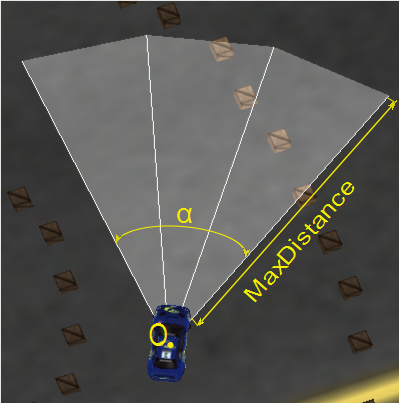
\includegraphics[width=0.38\textwidth]{visible-area}
  }\,
  \subfloat[Автомобіль застряг]{
  	\label{fig:car-stuck}
  	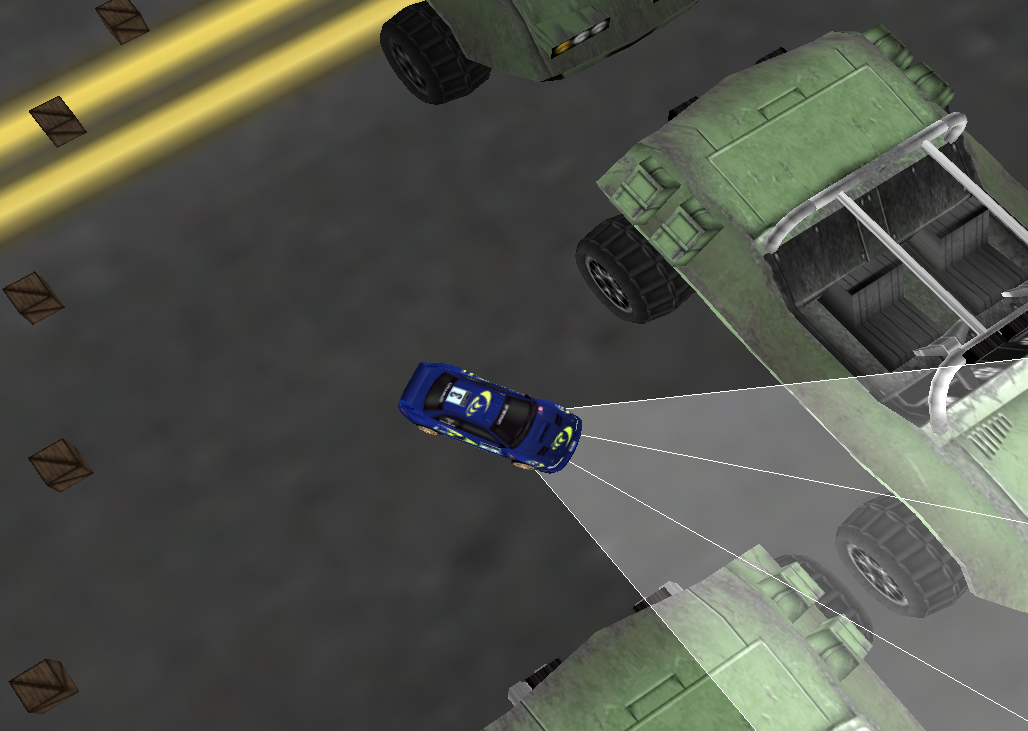
\includegraphics[width=0.54\textwidth]{car-stuck}
  }
  \caption{Ілюстрації до першого підходу}
  \label{fig:car-related}
\end{figure}

При використанні підходу з експертними правилами час вважався неперервним. Завданням агента був безперервний рух в межах середовища без натикання на нерухомі перешкоди. Як буде зазначено пізніше, при використанні самонавчання постановка задачі була дещо зміненою внаслідок особливості парадигми навчання з підсиленням.

\section{Експертні правила та штучна нейронна мережа}

Першим підходом до розв'язання задачі керування агентом було використання нейромережі з певним наперед заданим набором експертних правил. Експертні правила представляли собою пари відповідностей між вхідним вектором, який визначав певну еталонну ситуацію, та вихідним вектором керування, що являв собою бажану реакцію в такій ситуації. Ідея такого підходу полягає в тому, щоб використати нейромережу як універсальний апроксиматор функції. Надавши набір ключових правил, можна сподіватися на здатність нейромережі до узагальнення даних і використати цю властивість для поширення експертних знань на увесь простір можливих ситуацій. Таким чином, можна отримати контролер, який здатний приймати ``осмислені'' рішення в ситуаціях, для яких не було надано експертних правил, на основі правил, заданих для ``близьких'' ситуацій.

\subsection{Результати підходу на основі експертних знань}

Результати не можна охарактеризувати однозначно. З однієї сторони, система контролю на базі нейромережі досить адекватно керувала автомобілем з доволі складною фізикою, успішно оминаючи перешкоди та забезпечуючи безперервний рух автомобіля в середовищі, про яке вона не мала жодної попередньої інформації. Більше того, для підвищення рівня ``природності'' керування, системі контролю надавалася лише інформація про об'єкти, які попадали в поле зору автомобіля, що являло собою сектор з визначеним радіусом (дальністю бачення) та центральним кутом (кутом огляду). Базуючись лише на даних про віддаль до найближчих об'єктів в полі зору, система контролю забезпечувала завчасне оминання перешкоди з плавною зміною швидкості та напрямку руху автомобіля. Очевидно, що велику роль в досягненні вказаної природності та адекватності керування відіграла вдало підібрана навчальна множина.

З іншого боку, найбільшою проблемою, з якою довелося зіткнутися, була наявність ситуацій, в яких автомобіль зупинявся і система контролю не могла вивести його з нерухомого стану. Це, зокрема, ситуація, подана на рис.~\ref{fig:car-stuck}, в якій автомобіль заїхав у глухий кут і застряг, не зумівши здійснити розворот назад. Цю проблему, теоретично, можна було б розв'язати, ввівши у визначення стану автомобіля значення поточної швидкості та задавши додаткові набори ключових експертних правил, які б дозволили автомобілю здійснити розвертання у разі застрягання в глухому куті. Проте на практиці це достатньо проблематично, оскільки введення додаткової змінної стану призводить до ускладнення поведінки всієї системи, підвищення рівня вимог до точності та репрезентативності експертних правил. Більше того, для того, щоб зробити розвертання автомобіля безпечнішим та природнішим, довелося б вводити також змінні, які б відповідали за задній огляд автомобіля, що призводить до ще більш строгих вимог до експертних правил.

Слід зазначити, що ще однією причиною (окрім вказаної обмеженості визначеного стану динамічної системи) такої поведінки є особливість фізичної моделі автомобіля. Мається на увазі природа автомобіля "--- для того щоб здійснити поворот, чи, тим більше, розворот, автомобіль повинен здійснювати поступальний рух, що в умовах, коли вже відбулося ``застрягання'', дуже проблематично. Можливим розв'язанням даної проблеми є зміна типу транспортного засобу. Якщо взяти транспортний засіб, здатний здійснювати поворот без поступального руху, то можна значно зменшити ймовірність його застрягання. Таким транспортним засобом, для прикладу, може бути танк, в якому шляхом незалежного обертання гусениць
в різні сторони можна домогтися розвороту на будь-який кут, стоячи при цьому на місці.

Ще однією важливою проблемою є вибір внутрішньої структури нейромережі. Якщо використати недостатню кількість нейронів, то нейромережа не зможе в достатній мірі вивчити набір правил і, таким чином, не зможе в повністю використати експертні знання. З іншого боку, використовуючи надто велику кількість нейронів, існує загроза надто точного запам'ятовування (overfіttіng) правил без належної генералізації їх на схожі ситуації. В такому випадку нейромережа буде точно виконувати задані правила у відповідних ситуаціях, але навіть незначна зміна ситуації призведе до різкої зміни значень керованих змінних, порівняно з близькою еталонною ситуацією.

Таким чином, при використанні наперед заданих експертних правил, з'являється велика кількість практичних питань, на які немає чітких теоретичних відповідей, а все доводиться вирішувати в результаті численних експериментів. Саме тому було вирішено відійти від підходу, який базується на заздалегідь відібраних експертних знаннях, а піти шляхом самоорганізації "--- дати можливість агенту розробити власну систему правил на основі отриманого внаслідок взаємодії з середовищем досвіду.

\section{Самоорганізаційний підхід "--- навчання з підсиленням}

Оскільки використання попереднього підходу сильно залежить від якості навчальної вибірки (експертних правил), що при найменшому ускладненні сприйняття агентом середовища призводить до значних ускладнень експертних правил, було вирішено відійти від моделі навчання з учителем. Натомість був використаний самоорганізаційний підхід. Основна ідея такого підходу полягає в тому, щоб дати можливість агенту розробити власну систему правил щодо оптимальної поведінки в умовах середовища, завдяки безпосередній взаємодії з середовищем. Взаємодіючи з середовищем, агент отримує певний досвід і, якщо задати певний механізм оцінки агентом власних дій, то в результаті достатньої кількості ``досвіду'', можна надіятися, що агент розробить ефективну стратегію поведінки. Такий підхід отримав назву \emph{навчання з підсиленням (reіnforcement learnіng)}. При використанні навчання з підсиленням відпадає необхідність в досить складному і трудомісткому процесі розробки системи якісних і репрезентативних експертних правил, хоча, натомість, з'являється необхідність в виборі механізму оцінки дій агента. Проте, для достатньо складних систем зазвичай значно легше визначити механізм оцінки дій, аніж розробити достатньо повну та якісну систему правил.

Ми розглянемо застосування такого індуктивного процесу навчання (на відміну від дедуктивного на базі системи правил) до вищезазначеної задачі навігації агента в умовах наперед не відомого середовища, використавши принцип навчання з підсиленням (reinforcement learning).

\subsection{Загальні поняття навчання з підсиленням}

Ідея навчання з підсиленням полягає в наступному. Існує дві сутності "--- середовище та агент, що діє у ньому. Агент певним чином здатний сприймати середовище та має набір можливих дій, якими він здатний змінювати середовище. Уся сукупність інформації, доступна агенту в кожен дискретний момент часу $t$, називається \emph{станом} і позначається $s_t$. Відповідно можна ввести поняття множини усіх можливих станів середовища $\mathcal{S}\ (s_t \in \mathcal{S})$. Слід зазначити, що множина можливих станів може бути як дискретною, так і неперервною, а отже і нескінченною. При цьому в більшості реальних застосувань множина станів нескінченна. Також визначимо множину \emph{дій} агента, які допустимі в стані $s_t$ "--- $\mathcal{A}(s_t)$. Множина допустимих дій також в загальному випадку може бути нескінченною.

\begin{figure}
\centering
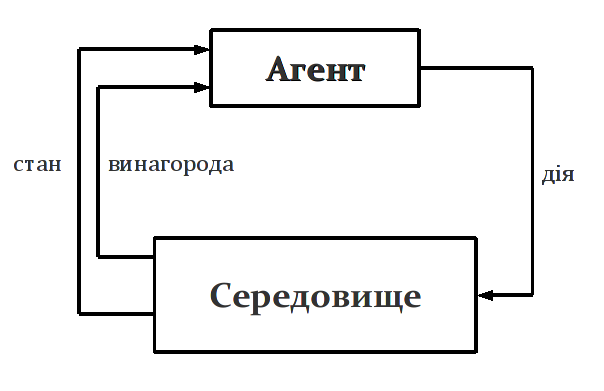
\includegraphics[width=0.5\textwidth]{agent-env-diagram.png}
\caption{Схема взаємодії агента та середовища}
\label{fig:agent-env-diagram}
\end{figure}
Схематично взаємодію агента та середовища представлено на рис.~\ref{fig:agent-env-diagram}. В дискретний момент часу $t$ агент отримує стан середовища $s_t \in \mathcal{S}$, на основі цієї інформації він вибирає і здійснює певну дію $a_t \in \mathcal{A}(s_t)$, в результаті чого отримує певне значення миттєвої винагороди $r_t \in \mathbb{R}$ від середовища. Метою агента в такій системі є визначення для кожної можливої ситуації $s_t$ такої дії $a_t$, яка приводить до максимізації сумарної винагороди в довготерміновому періоді (\emph{очікуваного прибутку} $R_t$). Більш формально це можна визначити так. Потрібно визначити відображення $\pi:\mathcal{S}\times\mathcal{A} \rightarrow [0,1]$, яке називається \emph{стратегією}, таке, що $\pi(s, a)$ визначає ймовірність здійснення дії $a$ при перебуванні агента у стані $s$. В випадку детермінованої стратегії, $\pi(s,a) \in \{0,1\}$. Стратегія $\pi$ називається \emph{оптимальною}, якщо для будь-якого стану послідовність дій, визначена нею, призводить до максимального очікуваного прибутку.

Визначимо більш точно поняття прибутку. Нехай, починаючи з часу $t$, агент отримує послідовність винагород $r_{t}, r_{t+1}, r_{t+2}, \ldots$. Тоді основною метою агента буде максимізація \emph{прибутку} $R_t$, де $R_t$ "--- це певна функція від послідовності винагород. В найпростішому випадку прибуток є сумою усіх винагород:

\begin{equation}
R_t = r_{t} + r_{t+1} + \cdots + r_T,
\end{equation}
де $T$ "--- кінцевий момент часу. Такий підхід до визначення прибутку підходить там, де можна природно визначити фінальний момент часу, тобто в таких системах, в яких взаємодія агента і середовища природно розбивається на окремі послідовності (\emph{епізоди}), наприклад, партії в грі, проходи по лабіринту або будь-який інший вид повторюваних взаємодій.

Кожен епізод закінчується у \emph{кінцевому (термінальному) стані}, після якого відбувається встановлення стану системи в певний початковий стан з множини можливих початкових станів і розпочинається наступний епізод. Задачі, в яких взаємодія агента і середовища відбувається у вигляді послідовності епізодів, називаються \emph{епізодичними задачами}. В епізодичних задачах інколи розмежовують множину усіх нетермінальних станів системи $\mathcal{S}$ та множину усіх станів, включно з термінальними "--- $\mathcal{S^+}$.

З іншого боку, не завжди можна здійснити природній поділ на епізоди, натомість взаємодія відбувається постійно без закінчення. Прикладом такої задачі може бути діяльність робота з великою тривалістю життєдіяльності. Такі задачі назвемо \emph{неперервними задачами}. В такому випадку кінцевий момент часу $T=\infty$, а сам прибуток, який ми намагаємося максимізувати, може легко прямувати до нескінченості (наприклад, якщо на кожному кроці $r_t=1$). Щоб подолати ці труднощі, введемо дещо інше визначення прибутку.

Розглянемо додаткову концепцію "--- \emph{зважування}. Згідно з нею, агент намагається вибирати такі дії, щоб максимізувати суму зважених винагород, які він отримає в майбутньому. Зокрема, агент вибирає таку дію $a_t$, яка максимізує очікуваний \emph{зважений прибуток}:

\begin{equation}
R_t = r_{t} + \gamma r_{t+1} + \gamma^2 r_{t+2} + \cdots = \sum_{k=0}^{\infty}\gamma^k r_{t+k},
\end{equation}
де $\gamma$ "--- це параметр зважування, $0\leq\gamma\leq 1$.

Таке зважування дозволяє регулювати важливість певної винагороди, залежно від віддаленості її у часі. Так, винагорода, отримана через $k$ кроків у майбутньому, ``важитиме'' у $\gamma^k$ раз менше, ніж якби вона була отримана безпосередньо на поточному кроці. З такого визначення прибутку видно, що якщо $\gamma<1$, то ця нескінченна сума має скінченне значення, якщо послідовність $\left\{r_k\right\}$ "--- обмежена. Якщо $\gamma = 0$, то агент є ``недалекоглядним'' і буде дбати лише про максимізацію миттєвої винагороди. Його задачею в такому випадку буде вибір такої дії $a_t$, щоб максимізувати лише винагороду $r_{t}$. Якщо дія агента не здійснює вплив на майбутні винагороди (наприклад, якщо система має лише один стан), то такий підхід дійсно дасть змогу вивчити оптимальну стратегію, однак в більшості випадків це не так, тому максимізація лише миттєвої нагороди може призвести до того, що буде втрачено нагоду ``заробити'' більше в майбутньому, здійснивши на даному кроці дію, яка принесе не максимальну миттєву винагороду. З наближенням $\gamma$ до 1 агент надаватиме майбутнім винагородам все більшого значення: агент стає більш ``далекоглядним''. Надалі припускатимемо використання саме зваженого прибутку.

Існують різноманітні методи навчання агента. Однією з найбільш вивчених у літературі є група методів, які базуються на побудові \emph{функції корисності} $V(s)$, яка визначає максимальний очікуваний прибуток для стану $s$. Серед цих методів можна виділити три категорії алгоритмів:

\begin{itemize}
\item методи динамічного програмування;
\item методи Монте-Карло;
\item методи часової різниці.
\end{itemize}

В даній статті ми розглянемо алгоритми, що належать до останної категорії, оскільки перші дві не є надто практичними для більшості реальних застосувань. Для більш детального ознайомлення можна звернутися до \cite{SuttonBarto2002}.

\subsection{Функція корисності}

Велика кількість алгоритмів навчання з підсиленням базується на оцінці \emph{функції корисності} "--- функції станів системи, що оцінює \emph{наскільки добре} для агента перебувати в заданому стані. Фраза ``наскільки добре'' визначається в термінах очікуваного майбутнього прибутку. Очевидно, що майбутні винагороди залежать від того, які дії здійснювати, тобто від стратегії, тому ціннісна функція визначається з врахуванням певної стратегії.

Нагадаємо, що стратегія $\pi$ "--- це відображення кожного стану $s \in \mathcal{S}$ та кожної допустимої дії $a \in \mathcal{A}(s)$ на ймовірність $\pi(s,a)$ здійснення дії $a$, будучи в стані $s$. \emph{Корисність} стану $s$ згідно стратегії $\pi$, $V^\pi(s)$,"--- це очікуваний прибуток, який можна отримати, якщо почати зі стану $s$ і діяти згідно стратегії $\pi$:
\begin{equation}
V^\pi(s) = E_\pi \Bigl\{ R_t \Big| s_t = s \Bigr \} = E_\pi \Biggl\{\sum_{k=0}^{\infty}\gamma^k r_{t+k} \Bigg| s_t=s \Biggr\},
\end{equation}
де $E_\pi{}$ позначає математичне очікування в випадку, якщо агент діє згідно стратегії $\pi$. Потрібно відмітити, що цінність термінального стану завжди рівна нулю. Назвемо функцію $V^\pi$ \emph{функцією корисності станів для стратегії $\pi$}.

Аналогічно, визначимо корисність здійснення дії $a$ в стані $s$ згідно стратегії $\pi$, $Q^\pi(s,a)$, як очікуваний прибуток, отриманий в результаті перебування в стані $s$, здійснення дії $a$ та подальшому слідуванні стратегії $\pi$:
\begin{equation}
Q^\pi(s,a)=E_\pi \Bigl\{ R_t \Big| s_t=s, a_t=a \Bigr\} = E_\pi \Biggl\{\sum_{k=0}^{\infty}\gamma^k r_{t+k} \Bigg| s_t=s,a_t=a \Biggr\}.
\end{equation}
Назвемо функцію $Q^\pi$ \emph{функцією корисності дій для стратегії $\pi$}.

Функції корисності $V^\pi$ та $Q^\pi$ можуть бути оцінені з досвіду. Наприклад, якщо агент притримується стратегії $\pi$ і підтримує середнє значення всіх прибутків, які були реально отримані, для кожного стану, в якому перебував агент, то середнє значення збіжиться до значення цінності для даного стану $V^\pi(s)$ за умови, що кількість перебувань в кожному зі станів прямує до нескінченності. Якщо зберігати середні значення окремо для кожної пари стан-дія, то таке ж твердження вірне і для функції $Q^\pi$. Такі методи оцінки цінових функцій називаються \emph{методами Монте-Карло}, тому що вони використовують усереднення по випадкових прикладах реальних прибутків. Проте, якщо кількість станів та можливих дій велика, це унеможливлює збереження середніх значень для кожного стану (пари стан-дія). В такому випадку можна застосувати інші методи, зокрема такі, що використовують апроксиматори функцій. Ми розглянемо їх дещо пізніше.

Фундаментальна властивість функцій корисності, яка використовується в навчанні з підсиленням і динамічному програмуванні,"--- це певне рекурсивне співвідношення, якому задовільняє функція корисності. Для будь-якої фіксованої стратегії $\pi$ та будь-якого стану $s$, наступне співвідношення завжди виконується:
\begin{eqnarray}
V^\pi(s) & = & E_\pi \Bigl\{R_t \Big| s_t = s \Bigr\} \nonumber\\
			& = & E_\pi \Biggl\{\sum_{k=0}^{\infty}\gamma^k r_{t+k} \Bigg| s_t = s \Biggr\} \nonumber\\
			& = & \sum_a \pi(s,a)\sum_{s'}\mathcal{P}^a_{ss'} \left[ \mathcal{R}^a_{ss'}+\gamma E_\pi \left\{\sum_{k=0}^{\infty}\gamma^k r_{t+k+1} \Bigg| s_{t+1} = s' \right\} \right] \nonumber\\
			& = & \sum_a \pi(s,a)\sum_{s'}\mathcal{P}^a_{ss'} \left[ \mathcal{R}^a_{ss'}+\gamma V^\pi(s') \right],
\label{Bellman_eq}
\end{eqnarray}
де $\mathcal{P}^a_{ss'}$ "--- це ймовірність переходу зі стану $s$ в стан $s'$ при виконанні дії $a$; $\mathcal{R}^a_{ss'}$ "--- очікувана винагорода, яка дається агенту при переході зі стану $s$ в стан $s'$ при виконанні дії $a$. В даній формулі неявно розуміється, що $s \in \mathcal{S}$, дії $a$ беруться з множини $\mathcal{A}(s)$, а $s' \in \mathcal{S}$ у випадку неперервної задачі або $s' \in \mathcal{S^+}$ "--- у випадку епізодичної задачі. Вказані ймовірності та очікувані винагороди визначають повну динаміку системи і на практиці зазвичай не відомі. Тому доводиться шукати методи, які б не потребували повних знань про систему.

Рівняння (\ref{Bellman_eq}) називається \emph{рівнянням оптимальності Белмана для $V^\pi$ (Bellman optіmalіty equation for $V^\pi$)}. Воно відображає зв'язок між корисністю стану $s$ та корисністю станів $s'$, в які можна потрапити з $s$. Можна довести, що функція $V^\pi$ "--- єдиний розв'язок рівняння Белмана. Відмітимо також, що це рівняння "--- основа для багатьох методів визначення наближень функції $V^\pi$.

\subsection{Оптимальні функції корисності}

Розв'язування задачі навчання з підсиленням означає, згрубша, знаходження такої стратегії, яка б давала великий прибуток в довгостроковій перспективі. Спробуємо визначити оптимальність стратегії наступним чином. Функції корисності визначають частковий порядок на множині усіх стратегій. Стратегію $\pi$ називатимемо \emph{кращою}, ніж стратегія $\pi '$, якщо її очікуваний прибуток більший або рівний від такого ж для стратегії $\pi '$ для усіх станів $s \in \mathcal{S}$:
\begin{equation}
\pi \geq \pi ' \Leftrightarrow \Bigl(\forall s \in \mathcal{S}\Bigr)\left\{ V^\pi(s) \geq V^{\pi '}(s) \right\}
\end{equation}

Завжди існує хоча б одна така стратегія, яка краща або рівна, ніж усі інші. Така стратегія називається \emph{оптимальною}. Хоча оптимальних стратегій може бути декілька, всіх їх будемо позначати як $\pi^*$. Усі оптимальні стратегії мають одну і ту ж функцію корисності станів, яка називається \emph{оптимальною функцією корисності станів} $V^*$:
\begin{equation}
V^* = \max_\pi V^\pi(s),\qquad \forall s \in \mathcal{S}.
\end{equation}

Оптимальні стратегії також мають одну і ту ж \emph{функцію корисності дій} $Q^*$:
\begin{equation}
Q^* = \max_\pi Q^\pi(s,a),\qquad \forall s \in \mathcal{S}, \forall a \in \mathcal{A}(s).
\end{equation}

Ми можемо також записати функцію $Q^*$ в термінах $V^*$:
\begin{equation}
Q^*(s,a) = E\left\{r_{t+1} + \gamma V^*(s_{t+1}) \Big| s_t=s, a_t=a \right\}.
\end{equation}

\subsection{Навчання з часовою різницею (TD-методи)}

Методи \emph{навчання з часовою різницею (temporal-dіfference, TD-навчання)} "--- це поєднання ідей методів Монте-Карло та динамічного програмування. TD-методи можуть, як і методи Монте-Карло, навчатися лише з досвіду, не потребуючи знання моделі динаміки середовища. З іншого боку, так само як і в методах динамічного програмування, TD-методи оновлюють свої оцінки частково на основі інших оцінок, не чекаючи закінчення епізоду.

Одними з найпростіших TD-методів навчання, які при цьому на практиці показують хороші результати, є \emph{Q-навчання} та \emph{Sarsa}.

Q-навчання є однокроковим алгоритмом навчання, який використовує функцію корисності дій, а не функцію корисності станів. При цьому правило оновлення оцінок значення Q-функції на кожному кроці виглядає наступним чином:

\begin{equation}
Q(s_t,a_t) \leftarrow Q(s_t, a_t) + \alpha \left[ r_t + \gamma \max_{a \in \mathcal{A}(s)} Q(s_{t+1}) - Q(s_t,a_t) \right].
\label{eq:q-update-rule}
\end{equation}

З (\ref{eq:q-update-rule}) видно, що значення Q-функції для поточного стану $s_t$ та виконаної дії $a_t$ модифікується з врахуванням винагороди, отриманої після виконання дії та максимальної зваженої сумарної винагороди (прибутку), яку можливо отримати зі стану $s_{t+1}$, в який було здійснено перехід. Проте, звісно, точне значення сумарних винагород нам не відоме, тому у всіх обчисленнями ми, фактично, використовуємо певні наближення, отримані з попереднього досвіду. 

Q-навчання добре розроблене в теоретичному плані, існують теореми, які доводять, що наближення Q-функції у границі при нескінченній кількості взаємодій з середовищем та нескінченній кількості оновлень кожної можливої пари $(s_t,a_t)$ збігаються до оптимальної $Q^*$-функції. 

Q-навчання є дуже простим для розуміння та теоретично обґрунтованим, проте часто на практиці значно краще себе показує інший алгоритм з родини TD-алгоритмів "--- Sarsa, який проте не має настільки хорошого теоретичного підґрунтя.  Sarsa, як і Q-навчання, апроксимує Q-функцію корисності дій на основі досвіду взаємодії з середовищем, проте використовує дещо інше правило оновлення наближень значення Q-функції:

\begin{equation}
Q(s_t,a_t) \leftarrow Q(s_t,a_t)  \alpha \left[ r_t + \gamma Q(s_{t+1}, a_{t+1}) - Q(s_t, a_t) \right].
\end{equation}

В даному випадку ми модифікуємо оцінку $Q(s_t,a_t)$ беручи до уваги не максимально можливий прибуток зі стану $s_{t+1}$, в який ми перейшли з $s_t$ шляхом виконання дії $a_t$, а лише той прибуток, який ми отримаємо, здійснивши у стані $s_{t+1}$ ту дію $a_{t+1}$, яка є оптимальною у стані $s_{t+1}$ згідно поточної стратегії вибору дій $\pi$. І хоч не зовсім зрозуміло, чому Sarsa дає кращі результати на практиці, проте можна відмітити, що після достатньої кількості ітерацій навчання, коли наближення Q-функції вже не будуть настільки випадково розподіленими, як на початку навчання, дія $a_{t+1}$ на наступному кроці все частіше буде оптимальною, тобто такою, що дає найбільший прибуток зі стану $s_{t+1}$. Таким чином, оновлення для Q- та Sarsa-навчання з часом будуть відбуватися однаково. Але при цьому Sarsa-навчання на практиці часто забезпечує швидшу збіжність Q-функції до оптимальної.

\subsection{Теоретичні умови збіжності}

В доведеннях теоретичної збіжності усіх вищезазначених методів роблять кілька суттєвих припущень, які не завжди виконуються на практиці. Порушення цих вимог може призвести як до лише незначного погіршення показників збіжності та ефективності навчання, так і до абсолютної непридатності вказаних методів до реальних задач. Нижче ми коротко розглянемо основні вимоги до вказаних методів.

\subsubsection{Процес прийняття рішень Маркова}

Ось як описується \emph{процес прийняття рішень Маркова (MDP)} в Wikipedia~(\cite{WikiMDP}):
\begin{quotation}
	Процеси прийняття рішень Маркова (MDPs), названі на честь Андрія Маркова, надають математичний апарат для моделювання прийняття рішень в ситуаціях, де результати є частково випадковими і частково залежать від особи, що приймає рішення. MDP корисні при вивченні широкого спектру оптимізаційних задач, які розв'язуються динамічним програмуванням або навчанням з підсиленням. MDP відомі принаймні з 1950-х років (згадуються в роботах Белмана).Сьогодні вони використовуються в різноманітних областях, включно з робототехнікою, автоматичним керуванням, економікою та у виробинцтві.

	Більш точно MDP можна визначити як стохастичний процес керування в дискретному часі, що характеризується множиною станів. Для кожного стану визначена множина дій, з якої особа, що приймає рішення, повинна вибирати. Для стану $s$ та дії $a$ функція переходу $P_a(s)$ визначає ймовірності переходу до наступного стану. ОПР отримує винагороду при кожному переході зі стану в стан. Цей перехід володіє властивістю Маркова: для будь-якого стану процесу в момент часу $t$ ймовірності переходу у стан в час $t+1$ є незалежними від усіх попередніх станів та здійснених дій.
\end{quotation}

Як видно з цього визначення, задача, яку розв'язує навчання з підсиленням, повністю задається в термінах MDP. Проте в реальних задачах дуже рідко повністю задовольняється вимога властивості Маркова. Це може бути як сама природа задачі, коли ймовірності залежать від попередніх станів та дій, так і просто неідеальність сприйняття стану, або ж просто неможливість взнати справжній стан системи (в цьому випадку говорять про значно складнішу задачу з частково спостережуваним MPD (POMDP). В першому випадку не виконується вимога незалежності розподілу ймовірностей переходів зі стану в стан від усіх попередніх станів та дій. В двох останніх випадках проблема полягає в тому, що ми не маємо справжнього стану $s$, який би повністю описував процес.

Ці питання потрібно враховувати при розв'язуванні конкретних задач. Проте, як показують численні практичні експерименти, незначне порушення властивостей MDP, не впливають суттєво на характеристики методів навчання з підсиленням.

\subsubsection{Стратегії вибору дій}
В усіх розглянутих алгоритмах потрібно на кожному кроці робити вибір дії, яку повинен здійснити агент. Це можна робити різними способами, проте, для збіжності стратегії до оптимальної, необхідною умовою є те, щоб кожна можлива дія була випробувана безліч раз при безмежній кількості ітерацій. Таку умову задовільняють так звані soft-стратегії, в яких ймовірність $\pi(s,a)>0,\ \forall \pi, \forall s \in \mathcal{S}, a \in \mathcal{A}(s)$.

Одним з найпростіших випадків soft-стратегії є $\varepsilon$-жадібна стратегія. В такій стратегії зазвичай вибирається дія, яка дає поточний максимум ціннісної функції, проте інколи, з ймовірністю $\varepsilon$, приймається рішення про здійснення довільної випадкової допустимої дії. Таким чином будь-яка не жадібна дія отримує ймовірність виконання, рівну $\frac{\varepsilon}{|\mathcal{A}(s)|}$, а жадібна дія, відповідно, $ 1 - \varepsilon + \dfrac{\varepsilon}{|\mathcal{A}(s)|}$.

Саме таку стратегію вибору дій було використано в цій роботі.

\subsubsection{Труднощі у випадку неперервного простору станів}

Якщо множина станів системи $\mathcal{S}$ дуже велика, як у випадку багатьох класичних ігор, або ж неперервна, то постає дуже важливе питання представлення функцій корисності. Існує багато варіантів вирішення цієї проблеми. І хоч ефективність кожного з методів сильно залежить від типу розв'язуваної задачі, одним з найбільш універсальних методів є лінійні та нелінійні апроксиматори функцій. При цьому лінійні апроксиматори, хоч і мають менші можливості, проте в більшості задач чудово справляються зі своїми завданнями і при цьому для випадку сумісного використання певних алгоритмів навчання з підсиленнями з лінійними апроксиматорами функцій були дані теоретичні гарантії збіжності до оптимальних стратегій при виконанні певних умов (\cite{Coulom2002}).

У випадку з нелінійними апроксиматорами, такими як штучні нейронні мережі, в силу їх більшої складності немає ніяких гарантій успішної збіжності до оптимальних стратегій. Більше того, для певних алгоритмів та задач було доведено, що використання нейромереж призводить до осциляції нейромережі (більш детальну інформацію можна знайти в \cite{SuttonBarto2002}). Тим не менше, нейромережі все ж таки успішно використовуються сумісно з різноманітними алгоритмами навчання з підсиленнями. Більше того, здатність нейромереж до узагальнення, дає можливість швидше навчати агента, оскільки визначивши вартість певного стану, вона певним чином наближає і вартості близьких станів. Таким чином потрібно менше ітерацій навчання для того, щоб функція корисності збіглася до оптимальної.

Як приклад одного з найуспішніших використань нейромереж у самонавчанні, можна навести програму TD-Gammon гри в нарди (backgammon), розроблену Gerald Tesauro (\cite{Tesauro1995}), яка в своїх останніх версіях грала на рівні з найкращими гравцями світу. Також успішні застосування нейромереж та методів навчання з підсиленнями можна знайти, наприклад, у \cite{Rummery1995} та \cite{Coulom2002}.

В даній роботі ми також використовували нейромережу як апроксиматор функцій і, як буде видно з результатів, досить успішно.

\subsection{Модифікація постановки задачі}

Для того, щоб більш ефективно використати навчання з підсиленням, були внесенні певні модифікації в формулювання задачі. Так, завдання агента було ускладнене "--- вимагалося, щоб агент не тільки оминав перешкоди, але й добирався до заданого пункту призначення.

При цьому, щоправда, були деякі спрощення. Так, час вважався дискретним. Також була спрощена фізика автомобіля. Тепер було можливо робити розворот на місці, що дозволяло уникнути проблеми застрягання, про яку вже згадувалося при огляді попереднього підходу. В силу цього було і спрощене керування. Для агента були доступні лише п'ять дій "--- рух вперед на певну фіксовану відстань, рух вперед з одночасним поворотом вліво або вправо на фіксований кут, а також поворот на місці вліво або вправо на фіксований кут. 

Вхідні дані були дещо розширені. Секторів огляду в агента стало 5, при цьому розміщувалися вони так, як показано на рис.~\ref{fig:tank-vis-area}. Таке розташування дає змогу сприймати об'єкти, що знаходяться дуже близько збоку, що покращує поведінку агента. Також агенту передавалася інформація про відстань до цілі та кут між напрямом руху агента та напрямком на ціль.
\begin{figure}
	\centering
	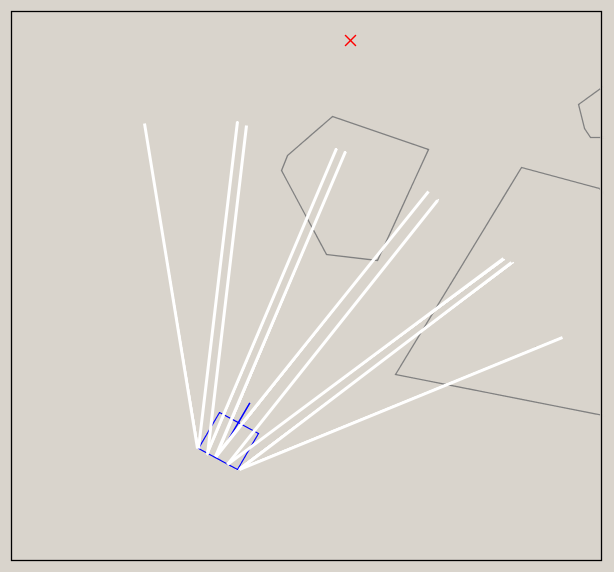
\includegraphics[width=0.4\textwidth]{tank-vis-area}
	\caption{Розташування секторів поля зору в модифікованій задачі}
	\label{fig:tank-vis-area}
\end{figure}

\section{Висновки}
\addcontentsline{toc}{section}{Література}
\begin{thebibliography}{99}
\bibitem{Rummery1995}{Rummery, G. A. 1995. Problem Solving with Reinforcement Learning. Ph.D. thesis. Cambridge University Engineering Department.}
\bibitem{SuttonBarto2002}{Sutton, R. S., Barto, A. G. 2002. Reinforcement Learning: An Introduction. A Bradford Book, The MIT Press, Cambridge, Massachusetts, London, England.}
\bibitem{Coulom2002}{Coulom, R. 2002. Reinforcement Learning Using Neural Networks, with Applications to Motor Control. Ph.D. thesis. Institut National Polytechnique de Grenoble.}
\bibitem{Kaelbling1996}{Kaelbling L., Littman M., Moore A. 1996. Reinforcement Learning: A Survey. Journal of Artificial Intelligence Research 4, 1996, 237-285}
\bibitem{Tesauro1995}{Tesauro G. 1995. Temporal Difference Learning and TD-Gammon. Communications of the ACM, March 1995 / Vol. 38, No. 3}
\bibitem{Kun03}{Phіlіppe Kunzle. Vehіcle Control wіth Neural Networks "--- http://www.gamedev.net/reference/artіcles/artіcle1988.asp}
\bibitem{WikiMDP}{Wikipedia. Markov Decision Process "--- http://en.wikipedia.org/wiki/Markov\_decision\_process}
\end{thebibliography}

\end{document}
